\documentclass[conference]{IEEEtran}
\usepackage[utf8]{inputenc}
\usepackage[T1]{fontenc}
\usepackage{graphicx,amsmath,amssymb,cite,url}
\usepackage[hidelinks]{hyperref}
\newenvironment{widefigure}[1][t]{\begin{figure*}[#1]}{\end{figure*}}
\newenvironment{widetable}[1][t]{\begin{table*}[#1]}{\end{table*}}

\newif\ifextended
\extendedtrue
\begin{document}
\title{Where to Put the Anchor: Synchronization Markers for Transformer-Based DNA Trace Reconstruction}

\author{
\IEEEauthorblockN{Hassan Ali\IEEEauthorrefmark{1}, Muhammad Haad\IEEEauthorrefmark{1}, Mahek Kalani\IEEEauthorrefmark{1}, and Muhammad Ismail Mangrio}
\IEEEauthorblockA{Department of Computer Science, Sukkur IBA University, Sukkur, Pakistan}
\thanks{\IEEEauthorrefmark{1}These authors contributed equally.}
}

\maketitle

\begin{abstract}
Deletions are the hardest errors in DNA data storage because they shift every later position of a read. We study
whether short synchronization markers, a classical tool from coding theory, help a deep-learning reconstruction model.
We fine-tune DNAFormer, a convolution--transformer network, on eleven designs of 128-nt strands that differ only in the
length, number and placement of their markers, and test them with 10 simulated reads per strand at deletion rates of
1--8\%. At 8\% deletion, four markers spread along the strand raise exact strand recovery from 38.8\% to 52.4\%, while the
same markers placed together at the end give no significant gain (41.0\%), so placement, not the shorter payload, drives
the effect. Eight 6-nt markers reach 69.6\%, and a single 6-nt marker in the middle gives the largest net data gain
(+12.5\%) at only 3.7\% cost when deletions are rare. Error-position profiles, a marker-scrambling ablation and
attribution maps (gradient$\times$input, Integrated Gradients, GradientSHAP) explain why: errors build up far from any
anchor, models trained with interior markers depend on them (scrambling the eight markers drops recovery from 69.6\%
to 18.4\%), and they draw on markers for nearby positions. Markers pay off only under heavy deletion.

\end{abstract}

\begin{IEEEkeywords}
DNA data storage, trace reconstruction, synchronization markers, deletion errors, transformers, explainable AI
\end{IEEEkeywords}

% Shared body for the IEEE and LNCS versions. Wide floats use the widefigure/widetable environments,
% which each main file defines (figure* / table* in IEEE, figure / table in LNCS).

\section{Introduction}

DNA can store digital data at very high density and for a very long time~\cite{church2012,goldman2013,erlich2017,organick2018}.
In a typical pipeline, data is encoded into many short synthetic strands, the strands are sequenced several times, and each
group of noisy reads of the same strand (a \emph{cluster}) is turned back into one estimate of the original strand.
This last step, \emph{trace reconstruction}, is hard because synthesis and sequencing introduce insertions, deletions and
substitutions. Deletions and insertions are the most damaging: a single missing nucleotide shifts every later position
of a read, so the reads of a cluster no longer line up~\cite{sabary2024}.

Deep learning has recently pushed trace reconstruction forward. DNAFormer~\cite{barlev2025} combines convolutional
alignment modules with a transformer~\cite{vaswani2017}, is trained on simulated clusters, and is fast and accurate
enough for large-scale storage. Like any reconstruction method, however, its accuracy falls quickly as the deletion rate
grows. In our simulations the pretrained model recovers about 90\% of 128-nt strands exactly at 5\% deletion but fewer
than 8\% at 8\% deletion.

Coding theory has a classical answer to synchronization errors: \emph{markers}, short known patterns inserted at fixed
positions so that a decoder can find its place again~\cite{sellers1962,davey2001,ratzer2005}. Marker codes have been
adapted to DNA storage~\cite{tong2023,haghighat2025}, but they are normally decoded with explicit, hand-designed
algorithms. It is not known whether a learned reconstruction model such as DNAFormer benefits from markers, how markers
should be placed and sized for it, and whether the model actually uses them.

This paper answers these questions with a controlled study. We fine-tune DNAFormer on eleven strand designs that differ
only in their markers and evaluate them under deletion rates from 1\% to 8\%. Our contributions are:
\begin{itemize}
  \item A controlled comparison with an \emph{end-block} control that holds the same marker nucleotides and the same
        amount of data as a spread layout, so that the effect of marker \emph{placement} can be separated from that of a
        shorter payload.
  \item A design study of marker length (4--12\,nt) and marker number (1--8 per strand), evaluated both by exact strand
        recovery and by \emph{net} data recovered, which charges markers for the space they take.
  \item An explanation of the effect: error-position profiles, a marker-scrambling ablation, and attribution maps
        (gradient\,$\times$\,input, Integrated Gradients~\cite{sundararajan2017} and GradientSHAP~\cite{lundberg2017}).
\end{itemize}
In short, markers placed inside the strand act as synchronization anchors that the model learns to rely on. At 8\%
deletion, four spread 8-nt markers raise exact recovery from 38.8\% to 52.4\%, whereas the same markers at the end of the
strand give 41.0\%. Eight 6-nt markers reach 69.6\%, and a single 6-nt marker in the middle gives the largest net data
gain (+12.5\%) at the lowest cost when deletions are rare.

\section{Related Work}

\textbf{DNA storage and reconstruction.} Early systems showed that megabytes of data can be written to and read from
DNA~\cite{church2012,goldman2013}, and later work added efficient coding~\cite{erlich2017} and random
access~\cite{organick2018}. Reconstruction algorithms estimate a strand from its noisy copies; Sabary et
al.~\cite{sabary2024} use dynamic programming over all traces. DNAFormer~\cite{barlev2025} replaces hand-designed
reconstruction with a siamese convolution--transformer network trained on simulated data and combines it with
tensor-product codes. We use DNAFormer as the reconstruction model and do not change its architecture.

\textbf{Markers for synchronization errors.} Sellers~\cite{sellers1962} inserted a known marker into a code word so that
a lost or gained bit could be located. Davey and MacKay~\cite{davey2001} proposed watermark codes for channels with
insertions, deletions and substitutions, and Ratzer~\cite{ratzer2005} showed that periodic marker codes concatenated with
LDPC codes work well at low insertion--deletion rates. For DNA storage, Tong et al.~\cite{tong2023} designed marker codes
at the nucleotide level, and Haghighat and Duman~\cite{haghighat2025} proposed half-marker codes that reserve one bit of
each base for synchronization. Ma et al.~\cite{ma2024} replaced the forward--backward marker detector with neural
networks. All of these use the markers explicitly in the decoder. We instead ask whether a general reconstruction
network, given marker-bearing strands, learns to use them by itself.

\textbf{Explaining sequence models.} Attribution methods assign each input feature a share of a model's output.
Integrated Gradients~\cite{sundararajan2017} integrates gradients along a path from a baseline, and
SHAP~\cite{lundberg2017} uses Shapley values, approximated for networks by GradientSHAP. We use the Captum
implementations~\cite{kokhlikyan2020} and complement them with an intervention (scrambling the markers), because
attributions alone show where a model looks but not whether that matters.

\section{Methods}

\ifextended
\begin{widefigure}[t]
  \centering
  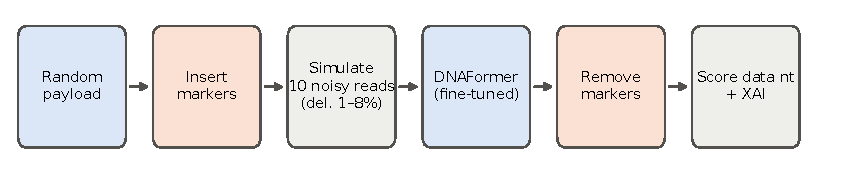
\includegraphics[width=\textwidth]{figures/fig_pipeline.pdf}
  \caption{Experimental pipeline. The same payloads and noise seeds are used for every design, so all designs are
  compared on identical random draws.}
  \label{fig:pipeline}
\end{widefigure}
Fig.~\ref{fig:pipeline} summarizes the pipeline.
\fi

\subsection{Data and strand designs}
Each cluster holds one 128-nt strand and 10 noisy reads. Payloads are uniformly random. Markers replace payload
positions, so a design with $m$ marker nucleotides stores $128-m$ data nucleotides (Table~\ref{tab:results},
Fig.~\ref{fig:layouts}). Reads are produced with the simulator released with DNAFormer~\cite{barlev2025}; each base is
deleted with probability $p_d\in\{1,3,5,8\}\%$, and insertions and substitutions occur with probability 1\% each
(single-base events only). The training set has 10{,}000 clusters (2{,}500 per deletion rate, mixed), the validation set
1{,}000, and each test set 1{,}000 clusters per deletion rate. All designs share the same payload seeds and noise seeds,
so cluster $i$ of every design comes from the same random draws; this allows paired statistical tests.

We study eleven designs. The \emph{spread} layouts divide the strand into $k$ equal blocks of data followed by a marker,
so the last marker sits at the end of the strand. The \emph{end-block} control places the same four 8-nt markers of the
spread 8-nt design together at the end: same marker content and same 96 data nucleotides, different placement. A
\emph{middle} layout places a single marker in the centre. Marker sequences were chosen to have no repeated adjacent
letter, no self-overlap, a GC content of 40--60\%, and a low occurrence in random payloads.
\ifextended
We enumerated all candidate $k$-mers for each length, removed those violating the first three rules, and ranked the rest
by how often they occur in the generated payloads. Repeating the ranking on two independently generated datasets gave
almost no agreement in rank among the valid candidates, as expected for uniformly random payloads; we therefore treat
the choice among valid candidates of one length as arbitrary and study length, number and placement instead.
\fi

\begin{figure}[t]
  \centering
  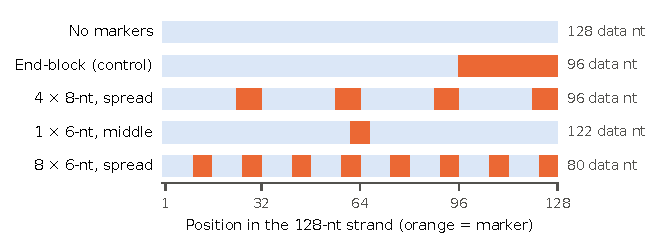
\includegraphics[width=\columnwidth]{figures/fig_layouts.pdf}
  \caption{Five of the eleven strand designs. Orange = marker nucleotides.}
  \label{fig:layouts}
\end{figure}

\subsection{Model and fine-tuning}
DNAFormer~\cite{barlev2025} reads up to 16 reads per cluster, each padded to 132 positions and one-hot encoded. A
siamese design processes the reads in forward and reversed order. Each branch has an alignment CNN (four parallel
kernels of size 1, 3, 5 and 7), an embedding CNN that sums over reads, a 12-layer transformer encoder (32 heads, model
width 1024) and a $1\times1$ convolutional output head; a learned per-position fusion combines the two branches
(103.4\,M parameters in total). We start from the authors' pretrained checkpoint and replace their data loader with one
that keeps every read (the original loader discards reads whose length differs from the design length, which removes
most reads at high deletion rates).

Every design is fine-tuned with identical settings: Adam ($\beta=(0.9,0.999)$), batch size 16, 10 epochs of 625 steps,
loss = cross-entropy + $0.25\times$ the consistency loss between the two branches, gradient clipping at 1.0 and mixed
precision. In epochs 1--2 the transformer is frozen (2.6\,M trainable parameters, learning rate $10^{-5}$); from epoch 3
the whole model is trained with a 100-step warm-up to $3\times10^{-6}$ followed by cosine decay to $10^{-7}$. The
checkpoint with the lowest validation edit distance on the data positions is kept. Training one design takes about
1.5\,h on a single NVIDIA T4 GPU.

\subsection{Metrics and statistics}
Markers are removed before scoring. \emph{Exact recovery} is the fraction of test strands whose data nucleotides are all
correct, with 95\% Wilson intervals~\cite{wilson1927}; we also report the normalized edit distance (NED). Because markers
take space, we define the \emph{net data recovered} per 1{,}000 strands as
\begin{equation}
  D = 1000 \cdot E \cdot n_{\mathrm{data}},
\end{equation}
where $E$ is the exact-recovery rate and $n_{\mathrm{data}}$ the number of data nucleotides per strand, and report it
relative to the marker-free design. Two designs are compared on the same 1{,}000 test strands with the exact McNemar
test~\cite{mcnemar1947}; differences in $D$ get a 95\% paired bootstrap interval (5{,}000 resamples). To check
reproducibility, three designs were trained a second time with a different seed.

\subsection{Explainability}
\textbf{Error-position profile.} For each strand position we count how often the model outputs a wrong nucleotide.

\textbf{Marker ablation.} For a trained model we replace every marker nucleotide of each test strand by a different random
nucleotide and regenerate the reads with the same noise seed, so the errors fall at the same places. Only the marker
letters change; the model is not retrained. The drop in exact recovery measures how much the model depends on its
markers.

\textbf{Attribution maps.} For 100 test strands at 8\% deletion we compute gradient\,$\times$\,input for each of the 128
output positions with respect to every nucleotide of every read. Each read is aligned to the true strand by edit
distance, so every read nucleotide is assigned a strand position; attributions are summed over reads, normalized per
output position and averaged, giving a $128\times128$ map. From the rows of data positions we compute the \emph{marker
share}, the fraction of attribution that falls on marker positions, and its ratio $\rho$ to the fraction of the strand the
markers occupy ($\rho=1$: attention in proportion to size). The marker-free model, scored on the positions of the
6-nt$\times$4 design, serves as a placebo. Integrated Gradients (32 steps, zero baseline) and GradientSHAP are computed with
Captum~\cite{kokhlikyan2020} on 20 strands per model, and the share of transformer attention on marker positions on 50.

\section{Results}

\subsection{Markers help only under heavy deletion}
Without fine-tuning, DNAFormer recovers 7.5--7.9\% of strands exactly at 8\% deletion for all three designs we tested (marker-free, spread 8-nt, end-block). Fine-tuning
raises the marker-free model to 38.8\% and benefits marker designs more. Table~\ref{tab:results} and
Fig.~\ref{fig:recovery} summarize all designs. At 1--3\% deletion every design recovers at least 99.5\% of strands. At
5\% the marker-free model already reaches 94.1\%, and markers add at most 3.3 points. At 8\% every spread design is
significantly better than the marker-free model ($p\le0.003$).

\begin{widetable}[t]
  \centering
  \caption{Fine-tuned DNAFormer on 1{,}000 test strands per deletion rate. Exact = strands with all data nucleotides
  correct (\%, 95\% Wilson interval at 8\%); layouts give data + marker nucleotides per block. $p$ = exact McNemar test against the marker-free design at 8\%.
  $\Delta D$ = net data recovered relative to the marker-free design (\%).}
  \label{tab:results}
  \footnotesize
  \setlength{\tabcolsep}{3.2pt}
  \ifextended\resizebox{\textwidth}{!}{\begin{tabular}{lrrrrrrr}
\hline
Design & Data nt & Exact 5\% & Exact 8\% [95\% CI] & $p$ (8\%) & NED 8\% & $\Delta D$ 8\% & $\Delta D$ 5\% \\
\hline
No markers & 128 & 94.1 & 38.8\,[35.8, 41.9] & -- & 0.0202 & -- & -- \\
End-block (control) & 96 & 95.7 & 41.0\,[38.0, 44.1] & 0.12 & 0.0241 & $-$20.7 & $-$23.7 \\
Spread 8-nt $\times$4 & 96 & 96.1 & 52.4\,[49.3, 55.5] & $6\times10^{-14}$ & 0.0148 & +1.3 & $-$23.4 \\
Spread 4-nt $\times$4 & 112 & 95.4 & 44.6\,[41.5, 47.7] & 0.001 & 0.0183 & +0.6 & $-$11.3 \\
Spread 5-nt $\times$4 & 108 & 95.6 & 45.7\,[42.6, 48.8] & $1\times10^{-4}$ & 0.0182 & $-$0.6 & $-$14.3 \\
Spread 6-nt $\times$4 & 104 & 95.3 & 49.6\,[46.5, 52.7] & $8\times10^{-10}$ & 0.0172 & +3.9 & $-$17.7 \\
Spread 7-nt $\times$4 & 100 & 96.1 & 49.9\,[46.8, 53.0] & $3\times10^{-10}$ & 0.0168 & +0.5 & $-$20.2 \\
Spread 12-nt $\times$4 & 80 & 97.1 & 62.3\,[59.3, 65.3] & $3\times10^{-35}$ & 0.0118 & +0.4 & $-$35.5 \\
Middle 6-nt $\times$1 & 122 & 95.1 & 45.8\,[42.7, 48.9] & $1\times10^{-5}$ & 0.0163 & +12.5 & $-$3.7 \\
Spread 6-nt $\times$2 & 116 & 95.4 & 43.7\,[40.7, 46.8] & 0.003 & 0.0179 & +2.1 & $-$8.1 \\
Spread 6-nt $\times$8 & 80 & 97.4 & 69.6\,[66.7, 72.4] & $1\times10^{-56}$ & 0.0096 & +12.1 & $-$35.3 \\
\hline
\end{tabular}
}\else\resizebox{\textwidth}{!}{\begin{tabular}{lrrrrrr}
\hline
Design & Data nt & Exact 5\% & Exact 8\% [95\% CI] & $p$ (8\%) & $\Delta D$ 8\% & $\Delta D$ 5\% \\
\hline
No markers & 128 & 94.1 & 38.8\,[35.8, 41.9] & -- & -- & -- \\
End-block (control) ($4\times8$, end) & 96 & 95.7 & 41.0\,[38.0, 44.1] & 0.12 & $-$20.7 & $-$23.7 \\
Spread, 8-nt ($4\times(24+8)$) & 96 & 96.1 & 52.4\,[49.3, 55.5] & $6\times10^{-14}$ & +1.3 & $-$23.4 \\
Spread, 4-nt ($4\times(28+4)$) & 112 & 95.4 & 44.6\,[41.5, 47.7] & 0.001 & +0.6 & $-$11.3 \\
Spread, 5-nt ($4\times(27+5)$) & 108 & 95.6 & 45.7\,[42.6, 48.8] & $1\times10^{-4}$ & $-$0.6 & $-$14.3 \\
Spread, 6-nt ($4\times(26+6)$) & 104 & 95.3 & 49.6\,[46.5, 52.7] & $8\times10^{-10}$ & +3.9 & $-$17.7 \\
Spread, 7-nt ($4\times(25+7)$) & 100 & 96.1 & 49.9\,[46.8, 53.0] & $3\times10^{-10}$ & +0.5 & $-$20.2 \\
Spread, 12-nt ($4\times(20+12)$) & 80 & 97.1 & 62.3\,[59.3, 65.3] & $3\times10^{-35}$ & +0.4 & $-$35.5 \\
Middle, 1 marker ($61+6+61$) & 122 & 95.1 & 45.8\,[42.7, 48.9] & $1\times10^{-5}$ & +12.5 & $-$3.7 \\
Spread, 2 markers ($2\times(58+6)$) & 116 & 95.4 & 43.7\,[40.7, 46.8] & 0.003 & +2.1 & $-$8.1 \\
Spread, 8 markers ($8\times(10+6)$) & 80 & 97.4 & 69.6\,[66.7, 72.4] & $1\times10^{-56}$ & +12.1 & $-$35.3 \\
\hline
\end{tabular}
}\fi
\end{widetable}

\begin{widefigure}[t]
  \centering
  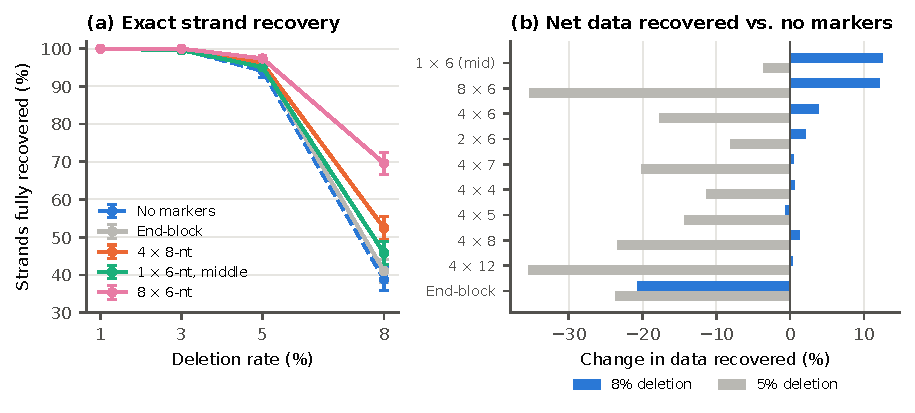
\includegraphics[width=\textwidth]{figures/fig_recovery.pdf}
  \caption{(a) Exact recovery versus deletion rate for five designs (95\% intervals). (b) Net data recovered relative to
  the marker-free design at 5\% and 8\% deletion. Markers pay for their space only at 8\%.}
  \label{fig:recovery}
\end{widefigure}

\ifextended
\textbf{Baselines.} Before fine-tuning we evaluated simple baselines on the marker-free, spread 8-nt and end-block designs.
Position-wise majority voting over the 10 reads fails completely (at most 3.6\% exact at 1\% deletion and 0\% from 3\%
on), because one deletion shifts the rest of a read. A majority vote that re-aligns the reads at each detected marker
recovers 53.4\% of strands at 1\% deletion and lowers the edit distance about tenfold, but still recovers none at 5\% or
8\%. Pretrained DNAFormer is near perfect at 1--3\% deletion (at least 99.8\%), reaches 88.5--91.2\% at 5\% and collapses to
7.5--7.9\% at 8\%, with overlapping confidence intervals for the three designs. Markers thus help a simple decoder directly, but a
learned decoder needs to be fine-tuned on marker-bearing strands before it can use them. Inference costs about 18\,ms per
cluster on a T4 GPU (batch 32, peak memory 0.7\,GB) for every design.
\fi

\subsection{Placement matters more than the markers themselves}
The spread 8-nt design and the end-block control carry the same 32 marker nucleotides and the same 96 data nucleotides.
At 8\% deletion the spread design recovers 52.4\% of strands and the end-block 41.0\% ($p=1.4\times10^{-9}$); the
end-block is not significantly better than having no markers at all (41.0\% vs.\ 38.8\%, $p=0.12$) and loses 20.7\% of
net data. The gain of the spread layout therefore comes from where the markers are, not from the shorter payload. At 5\%
deletion the two layouts do not differ ($p=0.69$).

\subsection{Marker length and number}
With four spread markers, exact recovery at 8\% rises with marker length: 44.6\% (4\,nt), 45.7\% (5\,nt), 49.6\% (6\,nt),
49.9\% (7\,nt), 52.4\% (8\,nt) and 62.3\% (12\,nt). Longer markers, however, take more space, so net data recovered stays
close to that of the marker-free design for all lengths ($-0.6$\% to $+3.9$\%, none significant).

With the 6-nt marker, accuracy rises with the number of markers: 43.7\% (two), 49.6\% (four) and 69.6\% (eight). At equal
marker space, many short markers beat fewer long ones: eight 6-nt markers recover 69.6\% against 62.3\% for four 12-nt
markers ($p=4.1\times10^{-5}$), also in net data (+5{,}840 per 1{,}000 strands, 95\% CI [3{,}120, 8{,}480]).
\ifextended
Fig.~\ref{fig:lennum} shows both trends.
\begin{figure}[t]
  \centering
  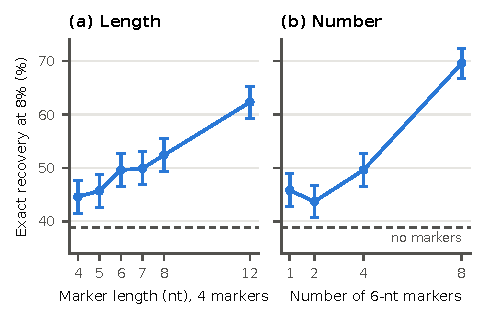
\includegraphics[width=\columnwidth]{figures/fig_length_number.pdf}
  \caption{Exact recovery at 8\% deletion versus (a) marker length with four spread markers and (b) the number of 6-nt
  markers (95\% intervals). Dashed: marker-free design.}
  \label{fig:lennum}
\end{figure}
\fi

Only two designs recover significantly more net data than the marker-free design at 8\%: one middle 6-nt marker
(+12.5\%, CI [+4.5, +20.2]\%) and eight 6-nt markers (+12.1\%, CI [+4.2, +20.0]\%); the two are indistinguishable in net
data. They differ sharply at low deletion: at 5\% the single marker costs 3.7\% of net data, eight markers 35.3\%.

\subsection{Reproducibility}
Retraining three designs with a second seed changed exact recovery at 8\% by 0.0 (marker-free), $+0.2$ (8-nt spread) and
$+1.2$ points (6-nt spread), none significant (McNemar $p\ge0.22$). The differences between designs reported above are
much larger than this run-to-run variation.

\section{Why Markers Help}\label{sec:why}

\subsection{Errors concentrate where the model is furthest from an anchor}
Without markers, errors form a single peak in the middle of the strand, reaching 14\% of strands at positions 60--70
(Fig.~\ref{fig:errors}). DNAFormer reads the cluster from both ends, so its position estimate is weakest far from either
end. With spread markers the error rate drops sharply right after each marker and grows again until the next one, a
saw-tooth pattern consistent with re-synchronization. The end-block profile follows the marker-free profile, because its
markers lie where errors are already rare. A single middle marker cuts the peak from about 14\% to 10\%, and eight
markers keep the error rate below about 4\% at every position.

\begin{widefigure}[t]
  \centering
  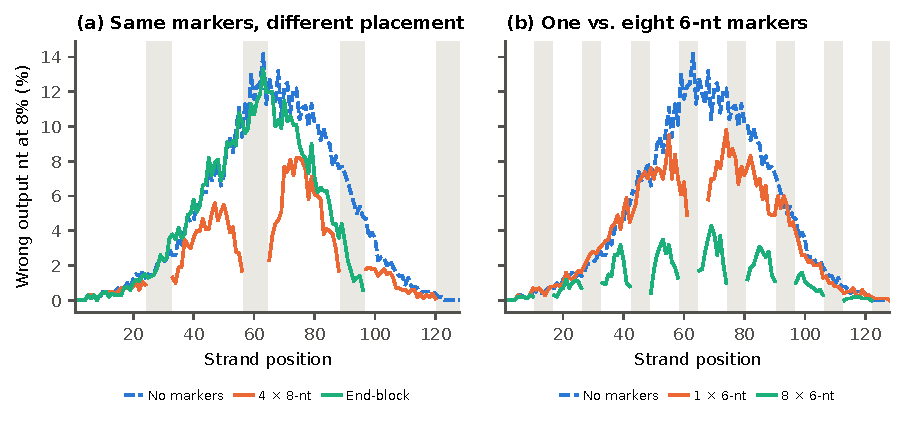
\includegraphics[width=\textwidth]{figures/fig_errors.pdf}
  \caption{Fraction of test strands with a wrong output nucleotide at each position (8\% deletion). Grey bands: marker
  positions of the spread 8-nt (a) and 8$\times$6-nt (b) designs; gaps are marker positions, which are not scored.}
  \label{fig:errors}
\end{widefigure}

\subsection{The model depends on its markers}
Scrambling the markers of a trained model changes nothing but the marker letters, yet recovery at 8\% falls sharply for
every spread design (Fig.~\ref{fig:ablation}, Table~\ref{tab:xai}): by 12.0 points for one middle marker, 17.8 for four
6-nt markers, 22.0 for four 8-nt markers and 51.2 for eight 6-nt markers (all $p<10^{-19}$). Every scrambled spread
model ends up \emph{below} the marker-free model (38.8\%), so the fine-tuned models have learned to rely on the markers
and are misled when they are wrong. Scrambling the 32-nt end-block costs only 3.8 points ($p=0.003$): six marker
nucleotides in the middle matter about three times more than 32 at the end.

\begin{figure}[t]
  \centering
  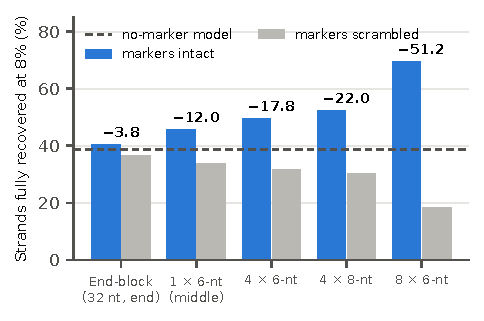
\includegraphics[width=\columnwidth]{figures/fig_ablation.pdf}
  \caption{Marker ablation at 8\% deletion: same model, same reads and noise, marker letters scrambled. Bold numbers:
  drop in percentage points. Dashed line: marker-free model.}
  \label{fig:ablation}
\end{figure}

\begin{table}[t]
  \centering
  \caption{Ablation drop at 8\% deletion and share of attribution on marker positions (data outputs only). Space =
  fraction of the strand occupied by markers; $\rho$ = gradient$\times$input share / space.}
  \label{tab:xai}
  \footnotesize
  \setlength{\tabcolsep}{2.6pt}
  \begin{tabular}{lrrrrrr}
    \hline
    Design & Drop & Space & G$\times$I & IG & GSHAP & $\rho$ \\
    \hline
    No markers (placebo) & -- & 18.8 & 18.4 & 17.5 & 17.6 & 0.98 \\
    End-block & 3.8 & 25.0 & 14.1 & 14.8 & 15.1 & 0.56 \\
    Spread 8-nt$\times$4 & 22.0 & 25.0 & 20.9 & 20.9 & 21.0 & 0.84 \\
    Spread 6-nt$\times$4 & 17.8 & 18.8 & 18.9 & 18.3 & 18.5 & 1.01 \\
    Spread 6-nt$\times$8 & 51.2 & 37.5 & 37.3 & 36.4 & 36.5 & 0.99 \\
    Middle 6-nt$\times$1 & 12.0 & 4.7 & 5.8 & 5.7 & 5.7 & 1.24 \\
    \hline
  \end{tabular}
\end{table}

\subsection{Where the model looks}
The attribution maps (Fig.~\ref{fig:heatmaps}) show a strong diagonal: each output position is computed mainly from the
aligned read positions around it, i.e., the model aligns the reads before deciding. Without markers the diagonal
broadens in the middle of the strand, where errors peak. With markers, thin vertical bands appear at the marker columns;
they are strongest where they cross the diagonal, i.e., for the data positions next to a marker. For the end-block, the
crossings fall on output positions 97--128, which are the markers themselves, so data positions draw little on them.

Table~\ref{tab:xai} quantifies this. The placebo gives $\rho=0.98$, so the measure is unbiased. The end-block receives
about half its share ($\rho=0.56$). Spread markers receive close to their share ($\rho=0.84$--$1.01$), and the single
middle marker receives more ($\rho=1.24$), consistent with it being the only anchor. Integrated Gradients and
GradientSHAP agree with gradient$\times$input within one percentage point for every model, so the conclusion does not
depend on the attribution method. Attributions show where the model looks; the ablation shows that this matters for the
output.

\begin{widefigure}[t]
  \centering
  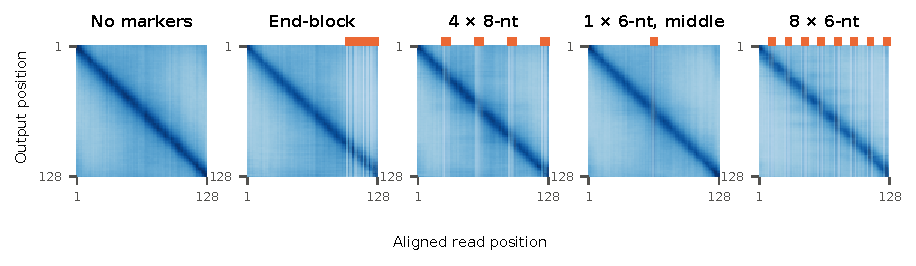
\includegraphics[width=\textwidth]{figures/fig_heatmaps.pdf}
  \caption{Gradient$\times$input attribution maps averaged over 100 test strands at 8\% deletion. Row = output position,
  column = aligned read position; darker = more attribution. Orange ticks: marker positions.}
  \label{fig:heatmaps}
\end{widefigure}

\ifextended
\subsection{A worked example}
Fig.~\ref{fig:example} shows one test strand at 8\% deletion for which the marker-free model fails and the middle-marker
model succeeds. The strand contains the run \texttt{CAC GGGG AATT} at positions 51--61. Three of the ten reads lost one
G of the run, so the reads disagree about where it starts. The marker-free model writes \texttt{C} in place of the first
\texttt{G}, its only error in the strand, and the strand is lost. The middle-marker model, whose marker begins four
nucleotides after the run, reconstructs every position. Among the first 300 test strands at 8\% deletion, 46 behave like
this one; the three clearest cases picked automatically all show a single wrong nucleotide near the middle of the strand
for the marker-free model. One example illustrates the mechanism; the statistics above establish it.
\begin{widefigure}[t]
  \centering
  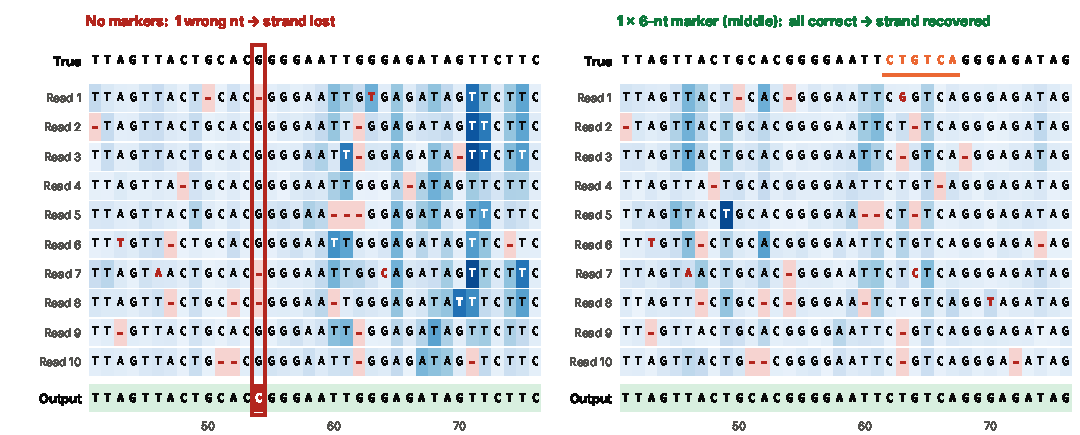
\includegraphics[width=\textwidth]{figures/fig_example.pdf}
  \caption{One test strand at 8\% deletion (positions 41--76). Rows: true strand, the ten aligned reads (red dash =
  deleted nucleotide, red letter = substitution, shading = gradient$\times$input) and the model output (red = wrong).
  Orange: marker. Inserted nucleotides are omitted to keep columns aligned.}
  \label{fig:example}
\end{widefigure}
\fi

\section{Discussion}

\textbf{Design guidance.} The results suggest three regimes. When deletions are rare (5\% or less), markers waste space
and the marker-free design stores the most data. When deletions are heavy and the goal is the most data per strand, a
single marker in the middle is best: it costs 4.7\% of the strand and gives +12.5\% net data at 8\% deletion while losing
only 3.7\% at 5\%. When complete strands matter most, for example to reduce the burden on an outer code, eight short
markers give the highest exact recovery (69.6\%). In every case markers should be placed where the decoder is weakest,
which for a bidirectional model is the middle of the strand, and many short markers are preferable to few long ones.

\textbf{Relation to marker codes.} Classical marker codes~\cite{sellers1962,ratzer2005} and their DNA
variants~\cite{tong2023,haghighat2025} require a decoder that explicitly searches for the markers. Here a general
reconstruction network, fine-tuned on marker-bearing strands for under two hours, learned to use the markers by itself,
and the ablation shows that it treats them as trusted anchors. This also means that markers must be synthesized reliably:
a model that relies on its markers is hurt more by corrupted markers than a model that never had them.

\textbf{Limitations.} All reads are simulated with independent single-base errors and a fixed coverage of 10 reads;
real nanopore or Illumina data have context-dependent and bursty errors. Most designs were trained once, although three
seed repeats varied by at most 1.2 points. We did not combine markers with an outer error-correcting code, so the effect
on end-to-end file recovery remains to be measured. In the spread layouts the last marker sits at the very end of the
strand, where Section~\ref{sec:why} shows it helps little; evenly spaced interior markers may perform better. Attribution maps are
averages over 100 strands and describe correlations; we therefore rely on the ablation for causal claims.

\section{Conclusion}

We studied whether synchronization markers help DNAFormer reconstruct DNA strands under heavy deletion. Spread markers
raise exact recovery at 8\% deletion from 38.8\% to up to 69.6\%, while the same markers placed at the end of the strand
give no significant gain, so placement is what matters. Error profiles, a marker-scrambling ablation and attribution maps
show why: errors build up far from any anchor, fine-tuned models depend strongly on interior markers, and they draw on
markers for nearby positions. A single middle marker gives the best net data gain at low cost, and eight short markers
give the most complete strands. Future work will test these designs on real sequencing data, combine them with outer
codes, and design reconstruction models that use markers explicitly.


\bibliographystyle{IEEEtran}
\bibliography{refs}
\end{document}
